\documentclass[11pt]{article}
%Gummi|065|=)
\usepackage[utf8]{inputenc}
\usepackage[spanish]{babel}
\usepackage{graphicx}
\title{\textbf{Código en python de los algoritmos práctica 3}}
\author{Javier Sáez, Laura Gómez, Daniel Pozo, Luis Ortega}
\date{}


\usepackage{listings}
\usepackage{color}

\definecolor{dkgreen}{rgb}{0,0.6,0}
\definecolor{gray}{rgb}{0.5,0.5,0.5}
\definecolor{mauve}{rgb}{0.58,0,0.82}

\lstset{frame=tb,
  language=Java,
  aboveskip=3mm,
  belowskip=3mm,
  showstringspaces=false,
  columns=flexible,
  basicstyle={\small\ttfamily},
  numbers=none,
  numberstyle=\tiny\color{gray},
  keywordstyle=\color{blue},
  commentstyle=\color{dkgreen},
  stringstyle=\color{mauve},
  breaklines=true,
  breakatwhitespace=true,
  tabsize=3
}

\begin{document}

\maketitle


\section{Ejercicio 1- Euler}
\begin{lstlisting}

import numpy as num
from decimal import *
import scipy as sci
from numpy.polynomial import polynomial as pol


def euler(f,a,b,n ,y_0):
    h=Decimal((b-a))/Decimal(n)
    vals = []
    vals.append(y_0)
    print ("Indice\t |  t  |  Aproximado(u) ")
    print("0\t |  0  |\t"+str(y_0)) 
    
    for i in range (0, n-1):
        tj =Decimal(a+(i+1)*h)
        x = vals[i] + h*f(tj,Decimal(vals[i]))
        vals.append(x)
        print(str(i+1)+"\t | "+str(tj)+" |"+"\t"+str(x))
        """print("u_",i+1,"=",x)"""


def f(t,x):
    return -x + t + 1

f0 = 1

euler(f,0,1,10,f0)
\end{lstlisting}
Vamos a ejecutarlo con la función $f = -x+t+1$
En el intervalo $[0,1]$ y con $n=10$.
El resultado es:
\begin{center}
  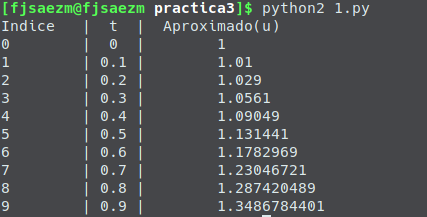
\includegraphics[scale=0.8]{1.png}
\end{center}

\section{Ejercicio 2 - Taylor de orden r}
\begin{lstlisting}
  # -*- coding: utf-8 -*-
import numpy
import itertools as it
from math import factorial
from sympy import symbols, diff, log
def genf(r, f, t ,y, t_s, y_s):
    faux = f
    for i in range(1, r):
        faux = diff(faux, t_s) + diff(faux, y_s)*f
        yield faux.subs(t_s,t).subs(y_s,y).evalf()

def T(t,y,h,f,r, t_s, y_s):

    suma = f.subs(t_s,t).subs(y_s,y).evalf()
    for i,f_i in enumerate(genf(r, f, t ,y, t_s, y_s)):
        suma += ((h**(i+1))/(factorial(i+2)))*f_i

    return suma

def taylor(f,a,b,n,y_0,r, t_s, y_s):
    uj = y_0
    h = float(b - a)/float(n)
    tj = float(a)
    print ("Indice\t |  t  |  Aproximado(u) \t| Real(y) \t\t| Error")
    for i in range (1, n+2):
        yield uj
        valor=func_y.subs(t,tj).evalf()
        print (str(i)+"\t | "+str(tj)+" |"+str(uj)+"\t|"+str(valor)+"  \t| "+str(valor-uj))
        uj = uj + h*T(tj, uj, h, f, r, t_s, y_s)
        tj = tj + h


t, y = symbols( 't y', real = True)

f = y**2/(1+t)

func_y= -1/log(t+1)

a = 1
b = 2
n = 10
y_0 = (-1/log(t+1)).subs(t,1).evalf()

print(f)
for i in taylor(f, a, b, n, y_0, 2, t, y):
    i
  \end{lstlisting}

Y si lo ejecutamos con $f=y^2/(1+t)$, y $[a,b]=[1,2]$, $n=10$ y $r=2$ obtenemos:
\begin{center}
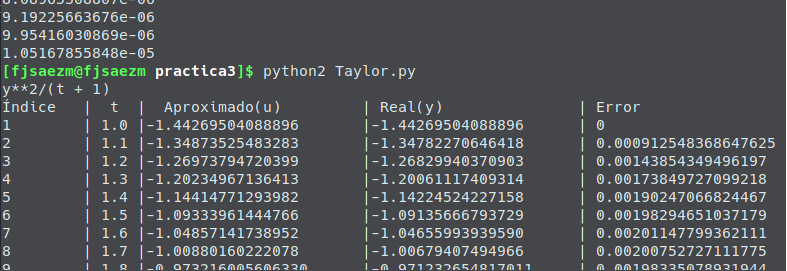
\includegraphics[scale=0.5]{Taylor.png}
  \end{center}
\section{Ejercicio 5 - Runge-Kutta }

\begin{lstlisting}
  # -*- coding: utf-8 -*-

import math

def RungeKutta(f,a,b,n ,y_0):
    h=float(b-a)/n
    vals = []
    vals.append(y_0)
    valor=y(1)
    print ("Indice\t |  t  |  Aproximado(u) | Real(y) \t\t| Error")
    print ("0\t |  1  |"+str(y_0)+"\t|"+str(valor)+"  \t| "+str(valor-y_0))
    """
        NOTA: Ahora mismo los valores tj se machacan con cada interacion y los
        valores aproximados u se almacenan en el vector vals.
    """
    for i in range (0, n-1):
        tj =a+(i+1)*h
        Ki = []
        Ki.append(f(tj,vals[i]))
        Ki.append(f(tj+h/2,vals[i]+(h/2)*Ki[0]))
        Ki.append(f(tj+h/2,vals[i]+(h/2)*Ki[1]))
        Ki.append(f(tj+h,vals[i]+h*Ki[2]))
        x = vals[i] + (h/6)*(Ki[0]+2*Ki[1]+2*Ki[2]+Ki[3])
        valor=y(tj)
        vals.append(x)
        print (str(i+1)+"\t | "+str(tj)+" |"+str(x)+"\t|"+str(valor)+"  \t| "+str(valor-x))


def f(t,x):
    return math.pow(x,2)/(1+t);

def y(t):
    return -1/math.log(t+1)

"""En t=1"""
f0 = -1/(math.log(2))

RungeKutta(f,1,2,10,f0)
  \end{lstlisting}
\section{Ejercicio 7}
\begin{lstlisting}
  import numpy as num
import scipy as sci
from decimal import *
from numpy.polynomial import polynomial as pol

def pMedio(f,a,b,n,y_0):
    h=Decimal((b-a))/Decimal(n)
    vals = []
    vals.append(y_0)
    print ("Indice\t |  t  |  Aproximado(u) ")
    print ("0\t |  0  |\t"+str(y_0))
    vals.append(euler1(f,a,b,n,y_0))
    print ("1\t | "+ str(h) + " |\t"+str(vals[1]))
    for i in range (2, n):
        tj = a+(i*h)
        x = vals[i-2] + Decimal(2*h*f(tj,vals[i-1]))
        vals.append(x)
        print(str(i)+"\t | "+str(tj)+" |\t"+str(x))



def euler1(f,a,b,n,y_0):
    h=Decimal((b-a))/Decimal(n)
    tj = Decimal(a+h)
    x = y_0 + h*f(tj,y_0)
    return x

def y(t,x):
	return -x*t + math.pow(t,2)/2 + t

def f(t,x):
    return -x + t + 1

f0 = 1

pMedio(f,0,1,10,f0)
\end{lstlisting}
Si lo ejecutamos con la misma función y otros parámetros del ejercicio 1, obtenemos:
\begin{center}
  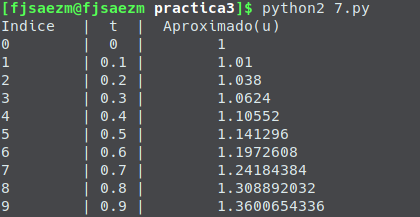
\includegraphics[scale=0.8]{7.png}
\end{center}

\section{Ejercicio 8- Adams-Bashforth}

\begin{lstlisting}
# PROGRAMA 8
# -*- coding: utf-8 -*-

from math import fabs, exp
from scipy.interpolate import lagrange
from scipy.integrate import quad

a = 0.0
b = 1.0
n = 10
k = 4

# Funcion f de dos variables
f = lambda t,y: -y + t + 1.0

# Solucion exacta
sol_exacta = True
y = lambda t: exp(-t) + t

# Lista con las aproximaciones u_{0},..,u_{k-1}
# (en caso de no tener la solucion exacta) 
inicial = []

h = (b - a) / n
t = [a + j * h for j in range(n + 1)]
u = [0 for i in range(n + 1)] # Lista "vacia" con n+1 posiciones

def integrate_interpolation_polynomial(j):
	x = []
	y = []
	for i in range(k):
		x.append(t[j-i])
		y.append(f(x[i], u[j-i]))

	poly = lagrange(x,y)
	return quad(poly, t[j], t[j+1])[0]
	
def adams_bashforth(j):
	if j < k:
		return u[j]
		
	u_j = adams_bashforth(j-1) + integrate_interpolation_polynomial(j-1)
	u[j] = u_j
	return u_j

"""
Main
"""

if sol_exacta:
	for i in range(k):
		u[i] = y(t[i])
else:
	for i in range(k):
		u[i] = inicial[i]

adams_bashforth(n)
print("Las", n, "aproximaciones son: ")
for item in u:
    print(item)
if sol_exacta:
    print("Los errores son: ")
    for j in range(n + 1):
        print(fabs(u[j] - y(t[j])))
\end{lstlisting}

Y si lo ejecutamos con $f=-y+t+1$,$[a,b]=[0,1]$,$n=10$, $k=4$ obtenemos:




\begin{center}
  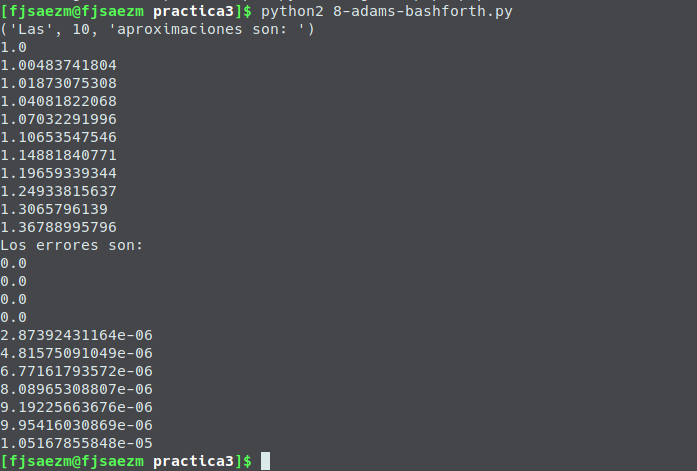
\includegraphics[scale=0.6]{8.png}
\end{center}
\end{document}
